\documentclass[16pt]{article}
\usepackage{fontspec}
\usepackage{parskip}
\usepackage{amsmath}
\usepackage{amssymb}
\usepackage{graphicx}
\usepackage{caption}
\usepackage{hyperref}
\usepackage{tabularx}
\usepackage{float}
\usepackage{subcaption}
\usepackage{algorithm}
\usepackage{algpseudocode}
\usepackage{algpascal}
\usepackage{geometry}
\usepackage{alltt}
\usepackage[backend=biber, citestyle=numeric, sorting=none]{biblatex}
\addbibresource{vde.bib}

\setmainfont{Noto Sans}
\hypersetup{urlcolor=blue, linkcolor=black, citecolor=black, colorlinks=true}
\author{James Engleback}

\begin{document}
\title{\textbf{VDE}}
\maketitle
\tableofcontents

\section{Abstract}
% ----------------
\section{Introduction}

\subsection{Background}
\subsubsection{Herbicide Resistant Crops}
Herbicide-resistant crops are important for global agriculture because they mitigate yield losses due to weeds and give farmers extra flexibility in their herbicide application programs, which is important to suppress emergence of herbicide-resistant weeds. 
% value statement

Herbicides kill plants by inhibiting key metabolic processes and their species-specificity is determined by susceptibility of herbicide target and their ability to  metabolize the herbicide. % herbicide overview
HPPD inhibitors are a key herbicide class that cause leaf bleaching and death in susceptible plants. 
HPPD inhibition  disrupts tyrosine catabolism which disrupts UV-protection via carotenoid production and photosynthetic electron shuttling via plastoquinone, leading to death by UV damage and radical toxicity. % HPPDs

Engineering HPPD-inhibitor resistance into plants have used the HPPD and metabolic enzymes from naturally resistant species like \textit{Avena fatua}, which employs cytochrome P450 Cyp72A1  to initiate metabolism of mesotrione by ring hydroxylation at $C_5$.
In this case, the $C_5$ hydroxylation acts as a target site for glutathione-S-transferases which conjugate glutathione to xenobiotics.
The glutathione conjugate tags the xenobiotic for sequestration in the cell vacuole, which neutralises the threat.

Engineered Cyp72A1 has been explored as a means of HPPD herbicide in soybean, which is an important target recipient for HPPD resistance traits. % cyp 72a1 & engineering attempts
%%%%% CYP71A1 stuff

\begin{figure}
	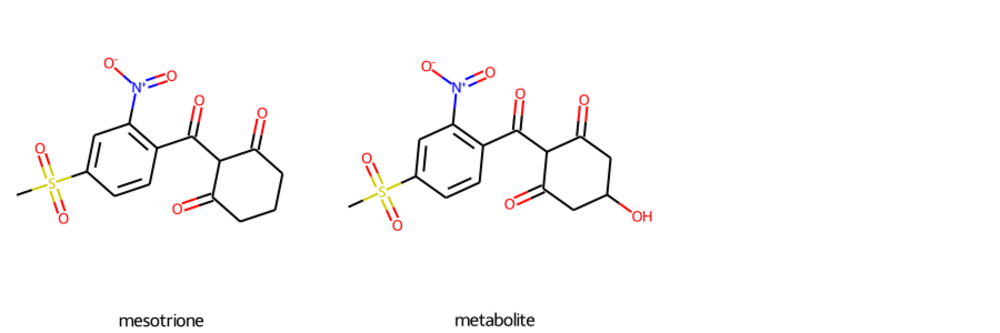
\includegraphics[width=\textwidth]{img/mesotrione+metabolite.png}
	\caption{\label{mesotrione} The HPPD inhibiting herbicide mesotrione and its primary metabolite 5-hydroxy-mesotrione in resistant strains of \textit{A. fatua}.}
\end{figure}

\subsubsection{Cytochrome P450s}
Cytochrome P450s are a ubiquitous class of heme-dependent oxido-reductases that are frequently involved in xenobiotic metabolism. % P450s overview
Bacterial P450s have been engineered to catalyse a range of xenobiotic biotransformations. 
The bacterial P450 BM3 from \textit{Bacillus megaterium} is one such bacterial P450 whose structure has been studied extensively. 
The A82F/F87V mutant has a broad substrate specificity, however it has no activity towards the HPPD herbicide mesotrione. % bacterial P450 engineering

\subsubsection{Virtual Directed Evolution}
Enzymes can be designed computationally using a genetic algorithm that evaluates the fitness of mutants by simulating the interaction between a target substrate and the predicted structure of the mutant. % computational enzyme edsign

The structure of a mutant can be predicted based on a template using techniques such as side-chain repacking by stochastic sampling from rotamer libraries and loop remodelling by cyclic coordinate descent. % structure pred - side chain repacking and loop ccd

% vde
Binding site interaction can be predicted using molecular docking, which attempts to predict likely protein-ligand binding conformations. 
A combination of the energy score and the conformation of docked molecules can be used to estimate likelihood of desirable reaction and therefore the fitness of a mutant. %score
In rounds of selection within a genetic algorithm, the fitness of a batch of mutants is evaluated by scoring desirability of protein-ligand binding, the fittest mutants are selected for breeding, in which mutants have elements of their genes recombined are further mutated, then the cycle repeats.   % genetic algorithms

\subsection{Technologies Used}
\subsubsection{Directed Evolution}
\subsubsection{Structure-Based Design}
\subsubsection{Protein Structure Prediction}
\subsubsection{Docking}
\subsubsection{Sequence Optimization Algorithms}
\subsubsection{Overview of this work}
\subsubsection{Engineering Problem}
\subsection{Overview of this Work}

Here, in attempt to engineer a mutant of the Cytochrome P450 BM3 to hydroxylate mesotrione at the $C_5$ position is made by developing a \textit{VDE} system, deploying it at scale on cloud infrastructure and identification on clusters of putatively active mutants.
% ----------------
\section{Methods}

The project was operated as a  \texttt{git} repository which can be found at:

\href{https://github.com/jamesengleback/vde}{https://github.com/jamesengleback/vde}.
The structure of the directory is:

\begin{itemize}
	\item \textbf{docs/:} write up for this document and markdown documentation
	\item \textbf{nb/:} jupyter notebooks used for data analysis
	\item \textbf{scripts/:} scripts to create and configure cloud machines to run algorithm on
	\item \textbf{vde/:} the vde algorithm configured to optimize BM3 for desirable mesotrione binding
\end{itemize}

This section details the implementation of this project:
\begin{itemize}
	\item The project is dependent on a \texttt{python} package \texttt{enz}, developed here for protein structure prediction and molecular docking to predict the behaviour of mutants; described in \ref{enz}.
	\item A score function that attempts to predict the likelihood of a $C_5$ hydroxylation of mesotrione is described in section \ref{scorefn}.
	\item A genetic algorithm to optimize the sequence of BM3 mutants is discussed in section \ref{ga} 
	\item Section \ref{cloud} describes execution of the algorithm at scale on cloud infrastructure.
\end{itemize}


% ---------------- enz ---------------- 
\subsection{\texttt{enz} \label{enz}}

Abstraction and modularization of protein structure prediction and molecular docking was important for reducing complexity of experiments and developability of the algorithm.
To this end the \texttt{python} package \texttt{enz} was created, an \textit{Application Program Interface (API)} wrapper around the \textit{PyRosetta} \cite{chaudhury2010pyrosetta} protein structure prediction software and the \textit{Autodock VINA} \cite{trott2010autodock} binary, as well as utilities to handle file format conversion using \textit{OpenBabel} \cite{o2011open}.
The package is modular enough to allow replacement of its functionality-providing back-ends according to a users requirements and is hosted at \href{https://github.com/jamesengleback/enz}{https://github.com/jamesengleback/enz}.

\texttt{enz} performs the following functions:
\begin{itemize}
	\item \textbf{Protein Structure Prediction:} \texttt{enz} uses side chain repacking \cite{dunbrack1993backbone} functionality from \textit{PyRosetta} for template-based structure prediction. 
		This functionality is provided by \textit{Pyrosetta}.
	\item \textbf{Docking:}
	\item \textbf{Return new atomic coordinates:} via \texttt{pandas} DataFrames, which can be used to score pose configurations.
\end{itemize}

The user-exposed command set is minimal so programs written using \texttt{enz} can be short.
Figure \ref{alltt} shows a short \texttt{python} program using \texttt{enz} to predict the structure of a new BM3 mutant, dock a fatty acid to it and save the results.
A key aspect not shown in \ref{alltt} is the accessibility of molecular data like coordinates, which are essential in this work for calculating distances between ligand and protein atoms and determining the score of the mutant.

\begin{figure}
	\caption{\label{alltt} A short program that uses \texttt{enz} to predict the structure of a BM3 mutant, dock a fatty acid to it and save the result.}
\begin{alltt}
        import enz 
        sequence = 'MKTIKEM...' 
        p = enz.protein('4KEY.pdb', 
                        seq=sequence, 
                        cofactors=['HEM']) \# 1. - initialization 
        p.mutate(181, 'S') \# 2. mutation
        p.mutate(87, 'A')
        p.refold() \# 3. refolding
        results = p.dock('CCCCCCCCCCCC=O',
                         target\_residues=[49, 75, 87, 181, 263, 330, 400]) \# 4. docking 
        results.save('docking-run-fatty-acid') \# save docking results
\end{alltt}
\end{figure}
% --------------- score -----------------
\subsection{Score function \label{scorefn}}
Given the aim of engineering a BM3 mutant capable of $C_5$ hydroxylation of mesotrione, and given that likelihood of electron transfer is proportional to $\frac{1}{d^6}$ \cite{moser2008distance}, the objective of the score function is to select for mutants that promote a mesotrione binding conformation where $C_5$ is close to the heme iron with a high affinity.
% whats a good distance in other crystal structures?
The $C_5$-heme iron distance is noted as $d$ measured in \AA.
Poses with a low $d$ should also be stably held with a low $\Delta G$, which is estimated for each pose by \textit{VINA}.

For a set of mutant-bound poses of mesotrione, their collective score could be:

\begin{equation}
	score = \frac{1}{n} \sum^{n}_{i\in n} \Delta G_{i} \times d_i
\end{equation}

Another important factor in the score function is the \textit{Hamming Distance} $h$ between the sequence of the mutant being scored and the template sequence.
Low $h$ can make DNA synthesis by a set of site directed mutagenesis reactions possible, or reduce the size of degenerate codon libraries by reducing the number of mutation sites.
A low $h$ is also important here because the structure prediction is purely template-based and a high $h$ could result in a very different structure in actuality.
So $h$ was added to the score function, which became score function $A$ to be used in experiment $A$ (equation \ref{scorea}).

\begin{equation}
	score = \frac{1}{n} \sum^{n}_{i\in n} d - \log{|\Delta G_{i}|} - h
\end{equation}

Low $\Delta G$ poses represent those more likely to occur, so their $d$ should be weighted according to $\Delta G$.



The heuristic currently employed to estimate the desirability of each set of $m$ docking results is described in equation \ref{scoreeqn}: % heuristic
\begin{equation}\label{scoreeqn}
	score = \frac{1}{n}\sum^{n}_{i\in m} \Delta G_{i} \times d_{i}
\end{equation}
where $\Delta G$ is a free energy estimation of the interaction calculated by \textit{Autodock VINA} (given in \textit{kcal/mol}) and $d$ is the distance between the heme iron and the $C_{5}$ of mesotrione for each of $m$ binding poses \textbf{(figure \ref{score})}. 

\begin{figure}
	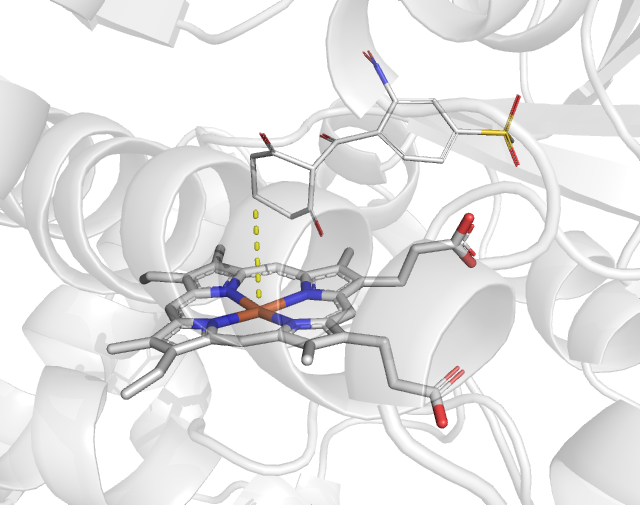
\includegraphics[width=\textwidth]{img/score.png}
	\caption{\label{score} - Distance $d$  between carbon $C_5$ of mesotrione and the heme iron of BM3, used in the fitness score (\AA) marked by a yellow dashed line.}
\end{figure}

\subsection{Genetic Algorithm \label{ga}}

A simple genetic algorithm \textit{(GA)} was used for sequence optimization during \textit{VDE}.
The \textit{GA} was implemented in pure \texttt{python} and its built-in modules.

In this case, the \textit{GA} repeated the following steps in each iteration:
\begin{enumerate}
	\item \textbf{Initialize mutant population:} From the template sequence, generate $p$ mutants each with one random point mutation.
	\item \textbf{For $n$ Iterations:}
		\begin{enumerate}
	\item \textbf{Evaluate \textit{fitness} of each mutant:\label{gaeval}} Using multiprocessing, evaluate the score for each mutant in parallel, returning a mapping of sequences to respective scores.
	\item \textbf{Select for best $\frac{1}{m}$ mutants:} where $\frac{1}{m}$ is the survival rate in each iteration.
	\item \textbf{Repopulate gene pool by crossover and point mutation of selected mutants:} where two random members of the surviving mutants $a$ and $b$ are crossed by recombining sequences at a random cut point and introducing additional random point mutation.
		Repeat $p$ times.
		\end{enumerate}
\end{enumerate}

\alglanguage{pseudocode}
\begin{algorithm}
	\caption{\label{pseudocode}: A genetic algorithm}
	\
	\begin{algorithmic}
		\Procedure{GA}{$sequence, n_{mutants}, n_{iter},n_{survivors}$} 
		\For{$i:=1; i < n_{mutants} ; i_{++}$} \Comment{Initialize a population of size $n_{mutants}$}
			\State $genePool_i := mutate(sequence)$  \Comment{Random substitution at random position}
		\EndFor
		\For{$i:=1 ; i < n_{iter} ; $} \Comment{For each generation}
			\ForAll{$mutant_j \in genePool$} \Comment{Map fitness function to each mutant}
				\State $fitness_j := fn(mutant_j)$  \Comment{where $fitness$ is mappable}
			\EndFor
			\State $genePool := nlargest(fitness,  n_{survivors}))$ \Comment{Select $n_{survivors}$ best sequences}
			\For{$i:=1 ; i < n_{mutants} ; i_{++}$} \Comment{Repopulate gene pool with new mutants}
				\State $newGenePool_i := mutate(crossover(genePool_{random}, genePool_{random}))$
			\EndFor
			\State $genePool := newGenePool$
		\EndFor
		\EndProcedure
	\end{algorithmic}
\end{algorithm}

Algorithm \ref{pseudocode} is implemented in \texttt{python} in the file \texttt{vde/ga.py} and makes use of multiprocessing to parallelise evaluations of a function.

\subsection{Main Function \label{main}}
The program in \texttt{vde/main.py} executes the main functionality of \textit{VDE}.
It executes iterations of the genetic algorithm \ref{ga} where the evaluation function for a $sequence $ is:

\begin{algorithm}
	\caption{\label{fitness}: One fitness evaluation}
	\begin{algorithmic}
		\Procedure{Evaluate Mutant}{$sequence$}
		\State structure = map\_refold(sequence, pdb=\texttt{4KEY.pdb}) \Comment{Predict mutant structure \cite{dunbrack1993backbone} \cite{chaudhury2010pyrosetta}.}
		\State docking poses = dock(structure, mesotrione) \Comment{\cite{trott2010autodock}}
		\State fitness = score(docking poses) \Comment{Using score \ref{scorefn}}
		\State \textbf{Return} fitness
		\EndProcedure
	\end{algorithmic}
\end{algorithm}

Two instances of the \textit{VDE} program were run, each with a different score function and labeled $A$ and $B$.
The score function for $A$ was as in equation \ref{scorea}:

\begin{equation}\label{scorea}
	fn_A(a, d, h) = d - \log{|a|} - h
\end{equation}

Where variables as in section \ref{scorefn}.
The score function for $B$ is described in equation \ref{scoreb}:

\begin{equation}\label{scoreb}
	fn_B(a, d, h) = (\frac{1}{n} \sum_{n}^{i} softmax(\log{|a|}_i)\times d_i) -  h
\end{equation}

Asides from the differing score functions, the two experiments were set up to be run with the configuration in table \ref{config}:

\begin{table}
        \begin{center}
		\caption{\label{config} The parameters used in experiments $A$ and $B$.}
                \begin{tabular}{l|p{3cm}}
		\textbf{Parameter} & \textbf{Value} \\
                \hline
			Template Structure & \textit{4KEY} \cite{butler2013key}\\
		Mutation Sites & 47, 49, 51, 75, 78, 88, 94, 138, 142, 175, 178, 184, 188, 205, 226, 252, 255, 260, 263, 290, 295, 328, 330, 350, 353 \\
		Population Size & 128 \\
		Survival Rate & $\frac{1}{4}$ \\
		Docking Exhaustiveness & 16 \\
		Number of Generations & 32 \\
		Number of Repeats & 8 \\
        \end{tabular}
        \end{center}
\end{table}

\begin{itemize}
	\item The \textit{Mutation Sites} were chosen manually from the crystal structure of P450 BM3 A82F/F87V mutant \texttt{4KEY} \cite{butler2013key}, the template structure for these experiments.
	\item \textit{Docking Exhaustiveness} is 16: the maximum value allowed by \textit{VINA}, which is computationally intensive but yields results with lower variability.
	\item \textit{Population Size} is 128, this was chosen because monitoring CPU usage was observed to be low in instances run with large \textit{Population Sizes} in a single process, so to maximize CPU usage, eight replicates were executed in separate parallel processes instead.

	\item \textit{Survival Rate} is $\frac{1}{4}$, where the top scoring fraction survive to repopulate the gene pool.
\end{itemize}

Experiment $A$ was run using code in the \texttt{git} branch \texttt{x2} on commit \texttt{????}, and experiment $B$ was run on branch \texttt{x3} and commit \texttt{e7af345fba8b8be36bea25982af0b978df8267e8}.

Each was run in eight parallel instances using the script \texttt{vde/vde.sh}, which launched \texttt{vde/main.py} with the command \texttt{python main.py -fn b -p 128 -e 16 -n 32 -s 0.25 \&}, which invokes the parameters in table \ref{config}.

% ---------------- cloud ----------------
\subsection{Cloud Deployment \label{cloud}}
Each \texttt{g6-dedicated-50} was provisioned with \texttt{evo/cloud/build-linode.sh} and the configuration scripts in \texttt{evo/scripts/config}.
The \textit{Linode} instance had the virtual hardware specifications showing in table \ref{linode}.

\begin{table}
        \begin{center}
		\caption{\label{linode} Virtual hardware specifications of the \texttt{g6-dedicated-50} server hired for experiments $A$ and $B$.}
                \begin{tabular}{l|p{3cm}}
		\textbf{Item} & \textbf{Specifications} \\
                \hline
			CPU cores & 50 \\
			RAM & 128 GB \\
			Disk & 250 GB \\
			Cost per hour & \$1.44 \\
        \end{tabular}
        \end{center}
\end{table}

Each experiment lasted about 3 days and cost \$103 at a rate of \$1.44 per hour. 
Data generated was structures, docking poses and scores for each mutant - it was compressed into a \texttt{.tar.gz} archive and uploaded to a \textit{Linode} bucket and the machines were terminated.

The eight replicates were run in parallel, generating 32,000 mutants for each experiment.

Data was pulled down from the bucket storage onto a separate server for analysis with specifications listed in table \ref{analysis}.
\begin{table}
        \begin{center}
		\caption{\label{analysis} Virtual hardware specifications of the \texttt{g6-dedicated-8} server hired for analysis of experiments $A$ and $B$.}
                \begin{tabular}{l|p{3cm}}
		\textbf{Item} & \textbf{Specifications} \\
                \hline
			CPU cores & 8 \\
			RAM & 16 GB \\
			Disk & 325 GB \\
			Cost per hour & \$0.18 \\
        \end{tabular}
        \end{center}
\end{table}

% ----------------
\section{Results}

Each experiment $A$ and $B$ yielded near to 32,000 unique mutants.
In each run, metrics were saved to a \texttt{csv} file containing the following headers:

\begin{itemize}
	\item \textbf{gene:} The mutant sequence represented only by the amino acids at the \textit{Mutation Sites} in table \ref{config}.
	\item \textbf{score:} The score $A$ or $B$ depending on which experiment is in question.
	\item \textbf{dist\_mean:} The mean distance between the $C_5$ carbon of a mesotrione pose and the heme iron, for all poses.
	\item \textbf{aff\_mean:} The mean binding energy estimate provided by \textit{VINA} for all poses, given in \textit{kcal/mol}
	\item \textbf{ham:} The Hamming distance, $h$ between a given mutant and the template sequence.
	\item \textbf{uid:} A unique ID.
\end{itemize}

The distributions for $A$ and $B$ are compared in figure \ref{abdistr}.
For both, there are many mutants for whom $d < 8$ which may be suitable for the project aim.

Between the two experiments, the distance $d$ between carbon $C_5$ and the heme iron is largely similar, so too are the calculated affinities ($\Delta G$) and Hamming distance to the wild type, $h$.
Hamming distance $h$ rarely exceeded 8, likely due to the constraint on $h$ incorporated into both score functions.
Docking binding energy estimates $\Delta G$ cluster at a set of values for both experiments which may indicate the same number of pose clusters with similar energies. 
For both, distance $d$ was a skewed distribution that leans towards lower values, each with a small shoulder at around 15 \AA, which may reflect either a cluster of binding poses or a cluster of mutants for which binding of mesotrione to the active site is blocked.

\begin{figure}
	\begin{center}
		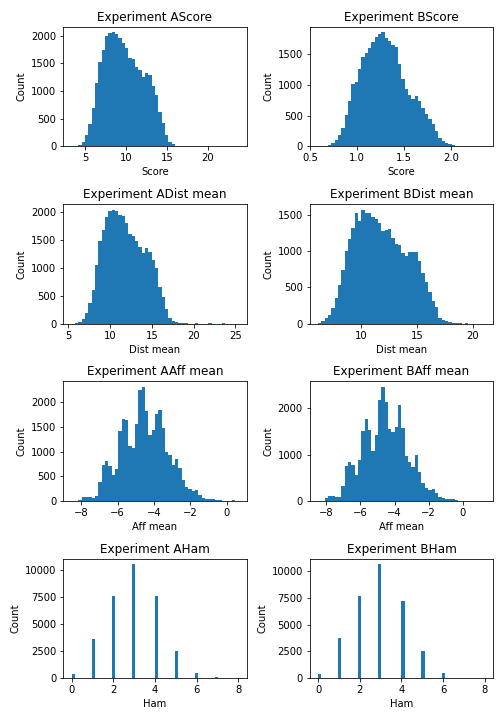
\includegraphics[width=0.7\textwidth]{img/exp-a-b-compr-dists.png}
		\caption{\label{abdistr} The distributions of each recorded metric across the entire experiment for both experiments $A$ and $B$.}
	\end{center}
\end{figure}

The repeats of each experiment converged towards a preferred mutation at each position.
Figure \ref{logot} is a sequence logo which shows the amino acids at each mutation site for the template sequence BM3 A82F/F87V, whilst \ref{logoa} and \ref{logob} represent the overall frequencies of different amino acids across experiments $A$ and $B$ respectively.
These mutations are shown in table \ref{mxntab}.

\begin{figure}
	\caption{\label{logos} Sequence logos.}
\begin{subfigure}{\textwidth}
	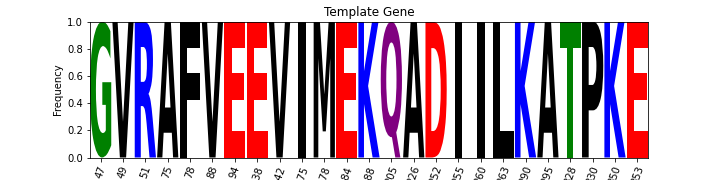
\includegraphics[width=\textwidth]{img/template-logo.png}
	\caption{\label{logot} Sequence logo showing the original amino acids at mutation positions in experiments $A$ and $B$.}
\end{subfigure}
\begin{subfigure}{\textwidth}
	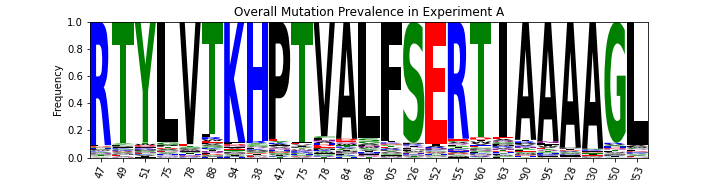
\includegraphics[width=\textwidth]{img/exp-a-logo.png}
	\caption{\label{logoa} Sequence logo showing the overall amino acid frequencies in mutants in $A$.}
\end{subfigure}
\begin{subfigure}{\textwidth}
	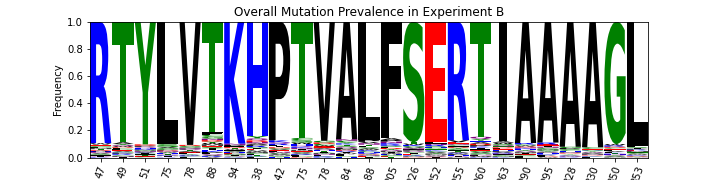
\includegraphics[width=\textwidth]{img/exp-b-logo.png}
	\caption{\label{logob} Sequence logo showing the overall amino acid frequencies in mutants in $B$.}
\end{subfigure}
\end{figure}

\begin{table}
        \begin{center}
		\caption{\label{mxntab} The mutations converged upon using \textit{Virtual Directed Evolution}}
		\begin{tabular}{l}
		\textbf{Mutation} \\
	    \hline
             G47R \\
             V49T \\
             R51Y \\
             A75L \\
             F78V \\
             V88T \\
             E94K \\
            E138H \\
            V142P \\
            I175T \\
            M178V \\
            E184A \\
            K188L \\
            Q205F \\
            A226S \\
            D252E \\
            I255R \\
            I260T \\
            L263I \\
            K290A \\
            A295A \\
            T328A \\
            P330A \\
            K350G \\
            E353L \\
\end{tabular}
        \end{center}
\end{table}

The exact set of 25 mutations in table \ref{mxntab} are never reached, since figure \ref{abdistr} shows that the \textit{Hamming Distance} $h$ never exceeded eight.
\textbf{Mutation Correlation}

Several clusters of mutants were identified using dimensionality reduction and clustering algorithms.
Mutant sequences were reduced in dimensionality using both the \textit{t-SNE} \cite{van2008visualizing} and \textit{UMAP} \cite{mcinnes2018umap} algorithms to decompose an input of the binary encoded  amino acids at each mutation position.
The reduced sequence information was plotted in two ways:

\begin{enumerate}
	\item Colour mapping score to each point, in an attempt to identify clusters with an especially high score (figure \ref{dimredplt}).
	\item Colour by point density (figure \ref{dimredds}).
\end{enumerate}

At the center of each dimensionality reduction map are the sequences that were repeatedly converged upon, visible by an area of low score (desirable).
When colored by point density the same low scoring centers of the mapping are also densely populated.
In order to confirm that the solutions in the centre were converged upon a generation number color map would be necessary, though was not possible since generation numbers were not recorded.

\begin{figure}
	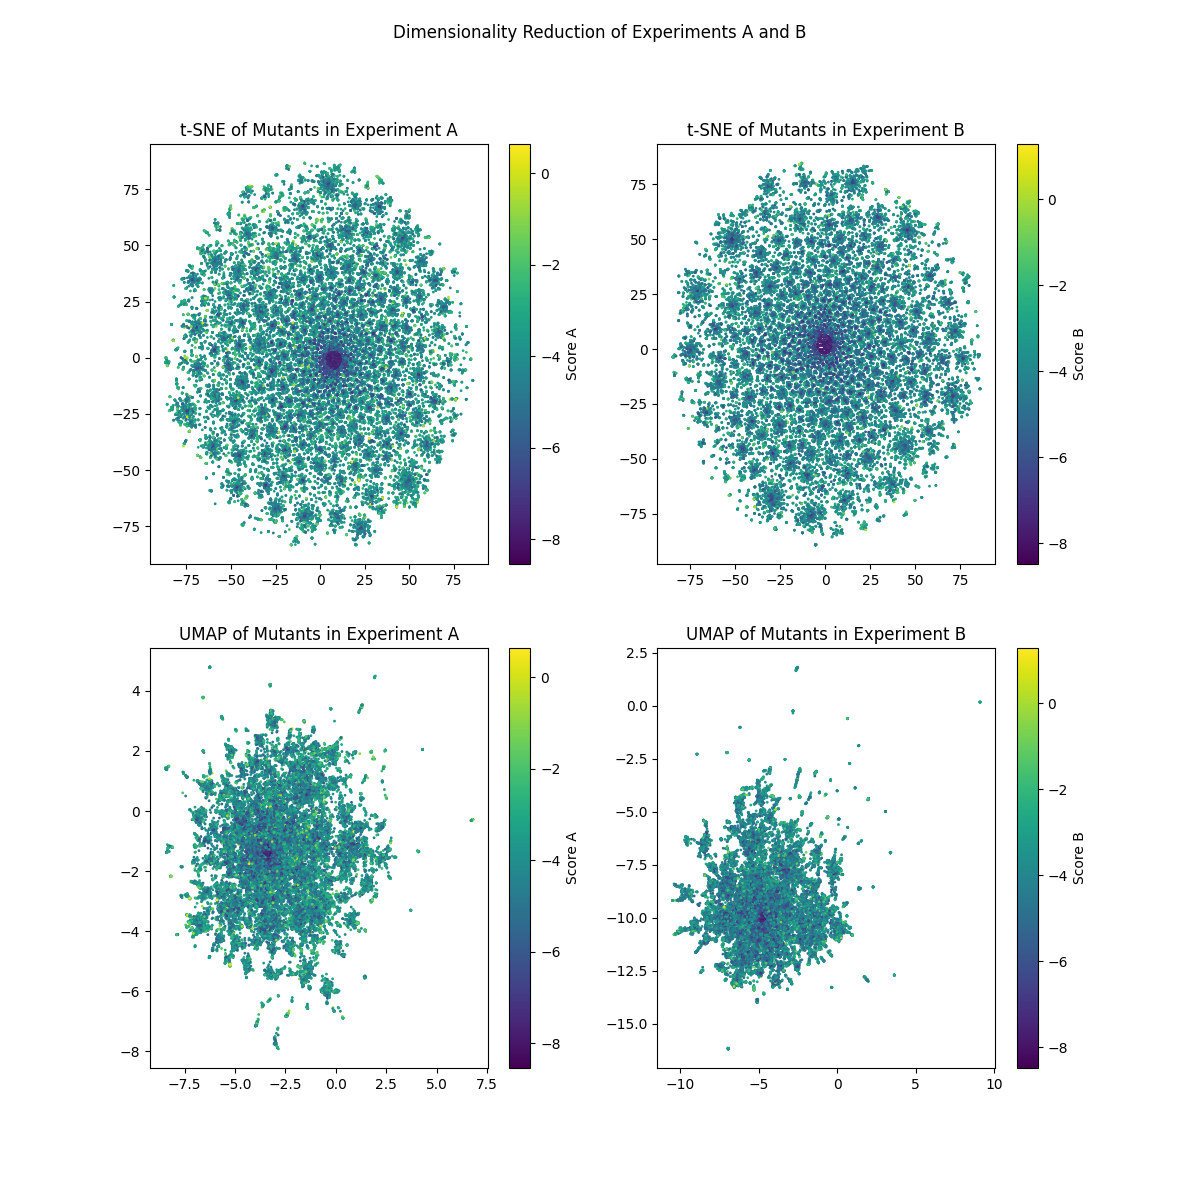
\includegraphics[width=\textwidth]{img/dimred-plt.png}
	\caption{\label{dimredplt}}
\end{figure}
\begin{figure}
	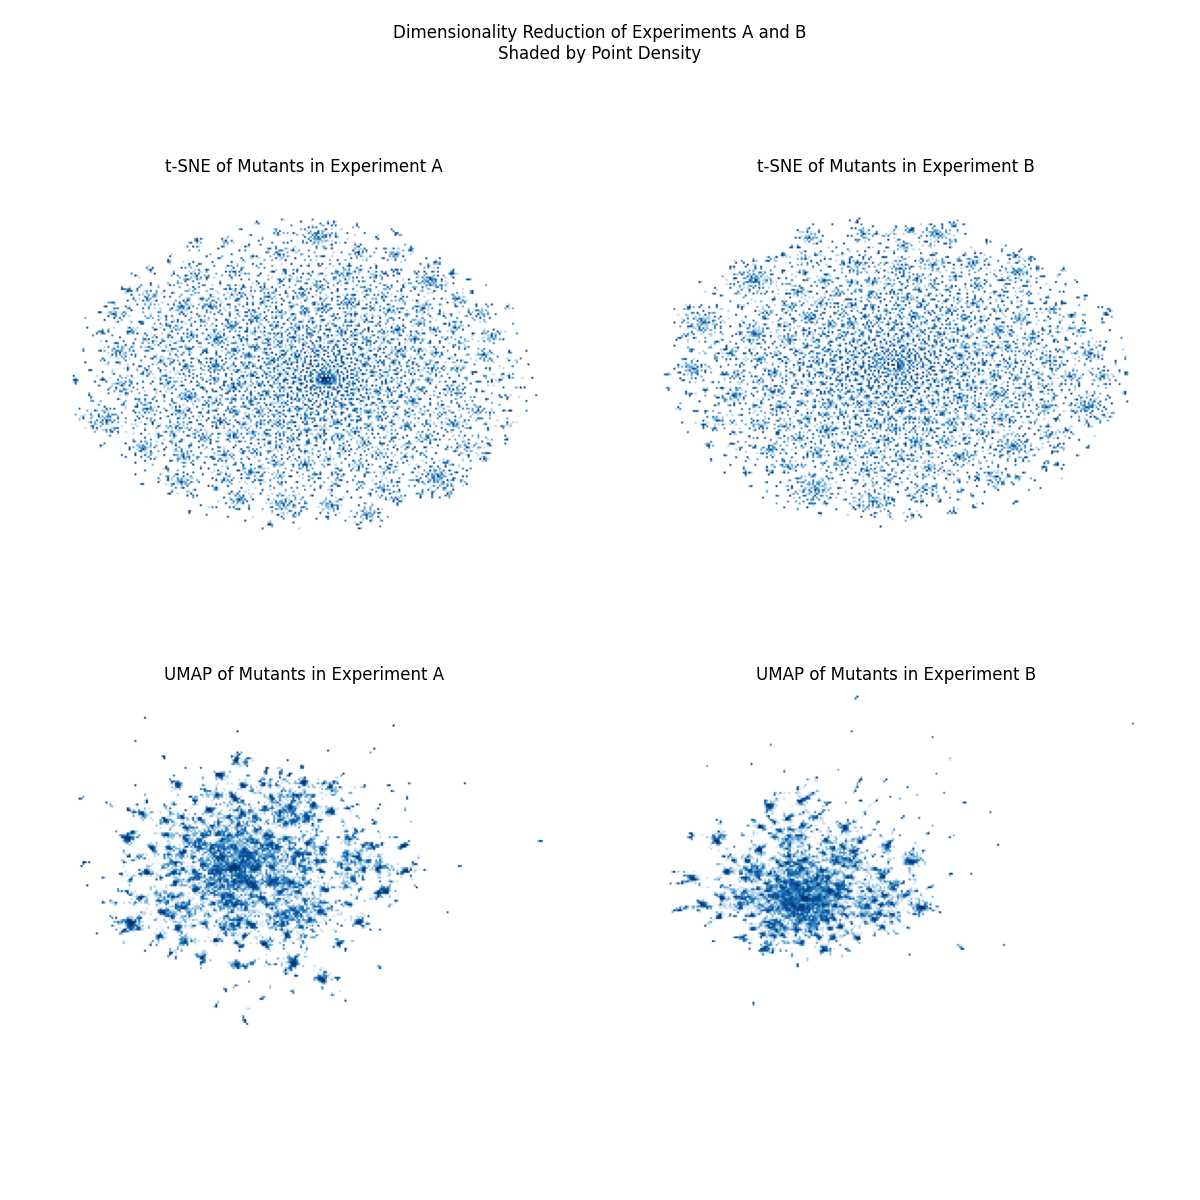
\includegraphics[width=\textwidth]{img/dimred-ds.png}
	\caption{\label{dimredds}}
\end{figure}

Whilst it is possible that the converged mutations are sufficient for creating a BM3 mutant with target activity, it is also possible that optimizing sequences for these scores exploited an inaccuracy in the model which would result in unintended consequences, such as large structural changes that can not be predicted by the model.
To mitigate the risk of a failed round of lab screening, it is prudent to identify other clusters with activity in order to introduce diversity into the screening set.
Clusters were made directly from the reduced dimensions using the \textit{DBSCAN} algorithm, exemplified in figure \ref{dimredclusters}.

\begin{figure}
	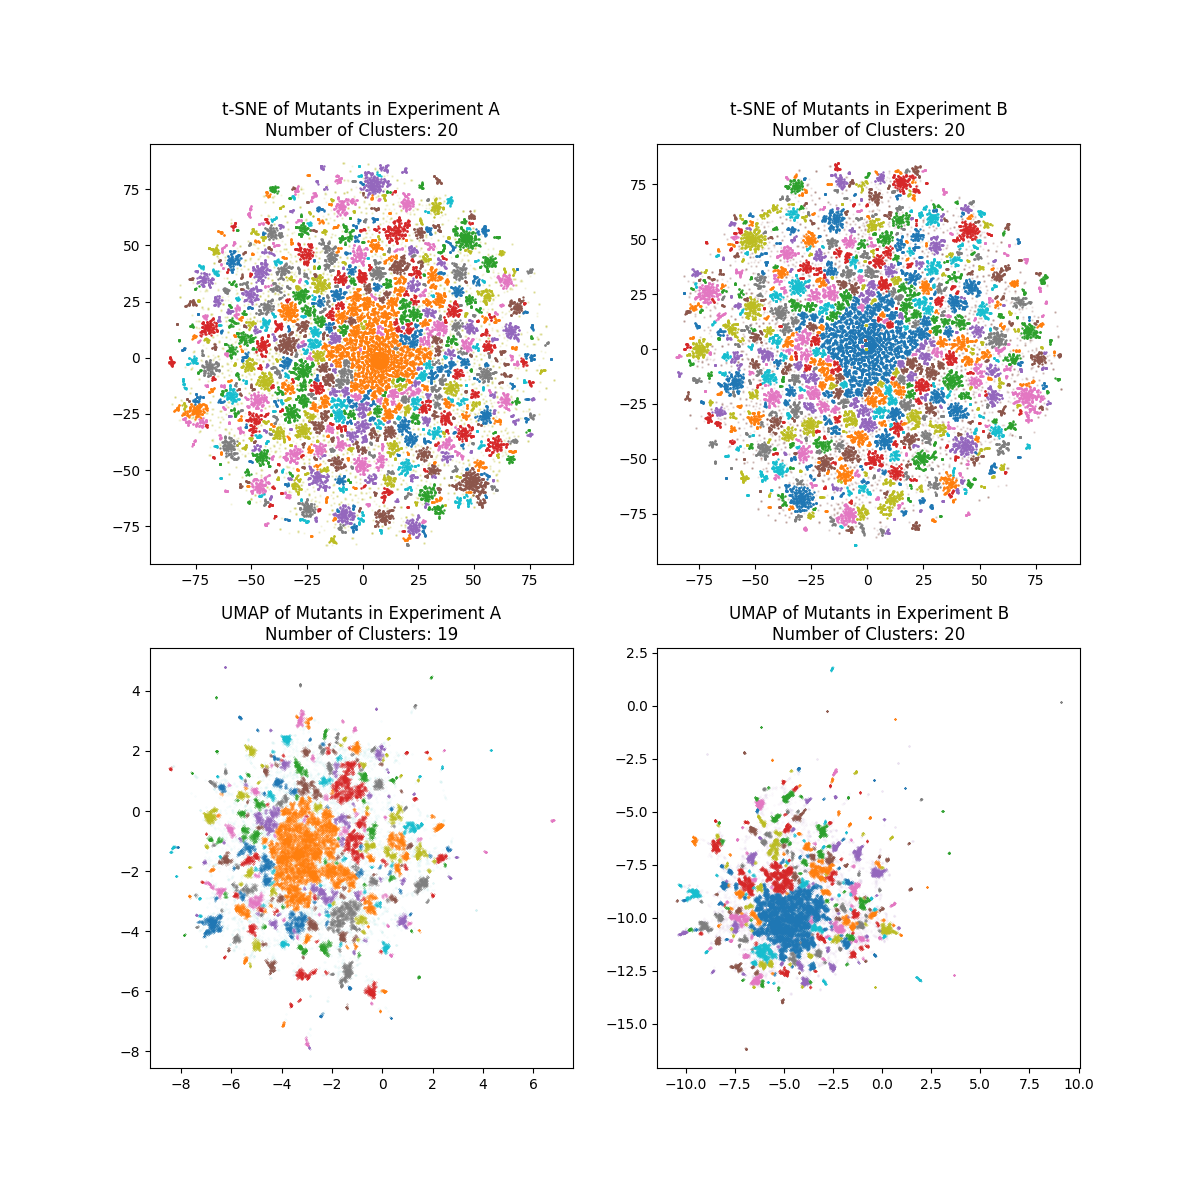
\includegraphics[width=\textwidth]{img/dimred-plt-clusters.png}
	\caption{\label{dimredclusters} Clusters of dimensionality-reduced mutants. Color codes to clusters are not shown.}
\end{figure}

From these clusters, the best scoring eight were selected, their amino acid frequencies calculated and degenerate codons designed to reflect that frequency using the \textit{Codon Genie API}.
Reports for each were generated and an example is shown in figure \ref{cdxreport}.


\begin{table}
\caption{\label{cdx314} An example of the codons auto-generated for mutant cluster 314, which encodes few variants. 
	A total of 1024 variants are encoded by this set of codons.}
\begin{tabular}{lllcl} 
	\textbf{Position} & \textbf{Codon} & \textbf{Expansion} & \textbf{Number of Encoded Variants} & \textbf{Amino Acids} \\
	\hline
	47  &   CGT &  CGT &       1 &  R \\
	49  &   ACC &  ACC &       1 &  T \\
	51  &   TAT &  TAT &       1 &  Y \\
	75  &   CTG &  CTG &       1 &  L \\
	78  &   GTT &  GTT &       1 &  V \\
	88  &   WSG &  ACG, AGG, TCG, TGG &             4 &  T, W, R, S \\
	94  &   AAA &  AAA &       1 &  K \\
	138 &   CAT &  CAT &       1 &  H \\
	142 &   GGT &  GGT &       1 &  G \\
	175 &   ACC &  ACC &       1 &  T \\
	178 &   GTT &  GTT &       1 &  V \\
	184 &   KMT &  GAT, GCT, TAT, TCT &             4 &  A, Y, D, S \\
	188 &   CTG &  CTG &       1 &  L \\
	205 &   TTT &  TTT &       1 &  F \\
	226 &   AGC &  AGC &       1 &  S \\
	252 &   GAA &  GAA &       1 &  E \\
	255 &   CAG &  CAG &       1 &  Q \\
	260 &   ACC &  ACC &       1 &  T \\
	263 &   MRT &  AAT, AGT, CAT, CGT &             4 &  N, R, H, S \\
	290 &   RMT &  AAT, ACT, GAT, GCT &             4 &  A, N, D, T \\
	295 &   GCA &  GCA &       1 &  A \\
	328 &   GCA &  GCA &       1 &  A \\
	330 &   RMA &  AAA, ACA, GAA, GCA &             4 &  A, K, E, T \\
	350 &   GGT &  GGT &       1 &  G \\
	353 &   CTG &  CTG &       1 &  L \\
\end{tabular}
\end{table}

The codons designed for exemplary cluster 314 are in table \ref{cdx314}.
In this manner codons were designed for clusters in experiments $A$ and $B$, the data and reports for which are stored in \texttt{nb/codons/} of the project \texttt{git}  repository.
The total size of each library yielded by the codon design varies from four to several thousand, the latter of which are not suitable for use owing to the extreme numbers of potential variants.
Some libraries also inadvertently encode a \textit{Stop} codon, which should also be avoided.


\begin{figure}
\begin{subfigure}{\textwidth}
	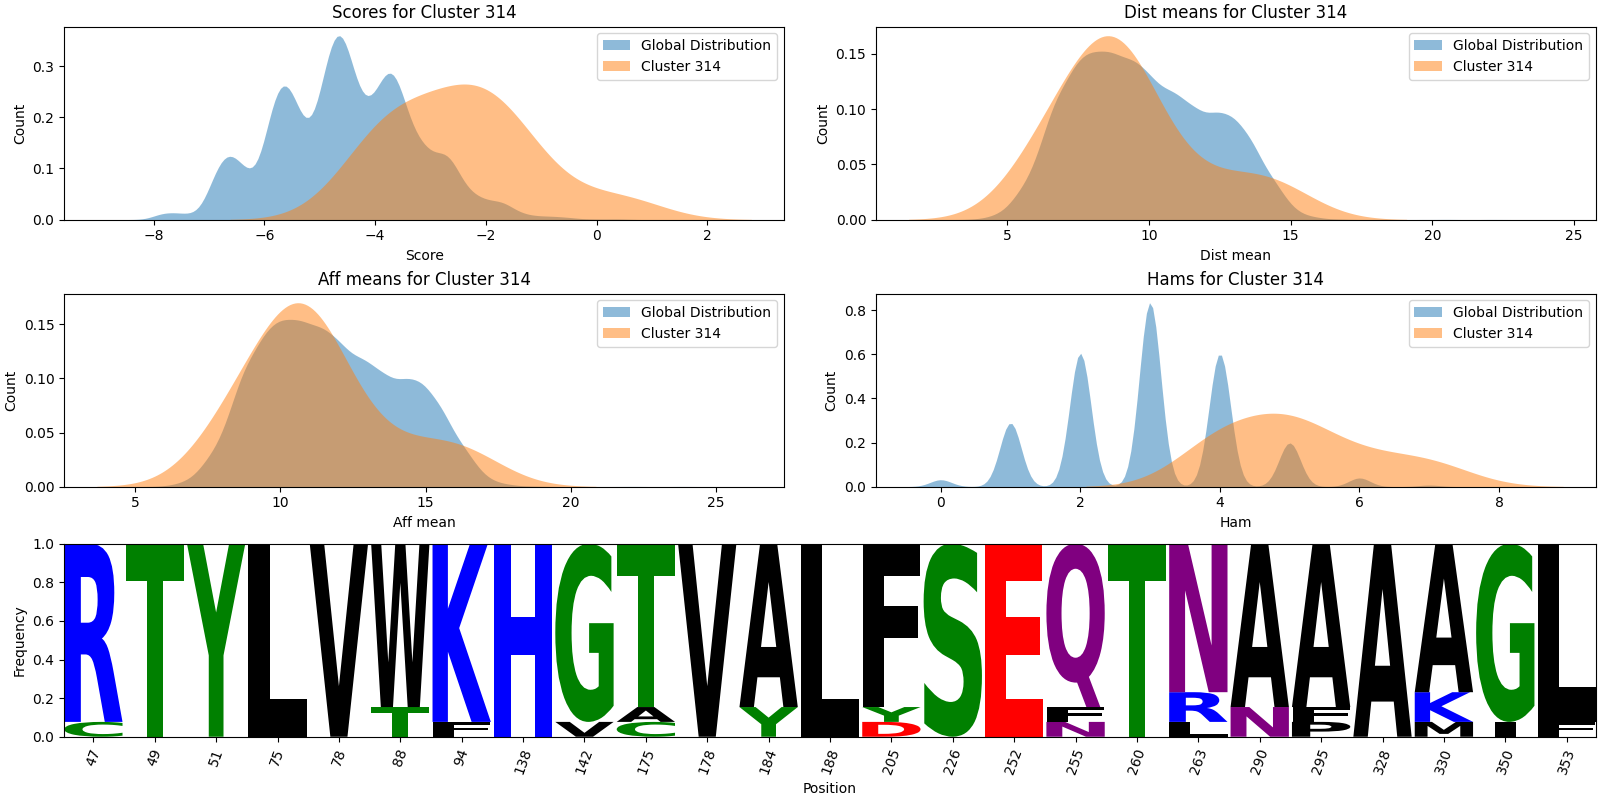
\includegraphics[width=\textwidth]{img/clus_314.png}
	\caption{\label{cdxreport} A codon report for cluster 314 derived from a \textit{UMAP} of the sequences in experiment $A$.
		 Shown are the cluster distributions of each recorded metric relative to the global distribution.
		 The sequence logo represents the mutation frequency at each position.}
\end{subfigure}
\begin{subfigure}{\textwidth}
	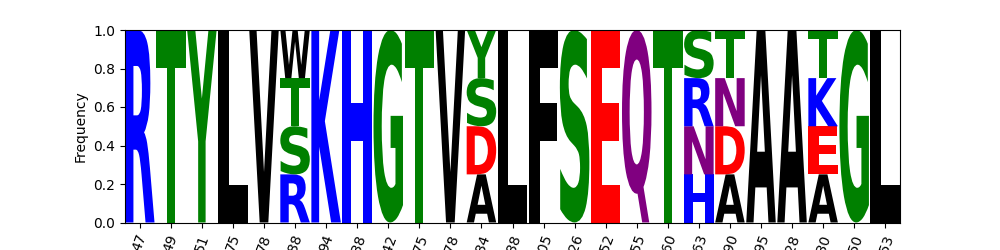
\includegraphics[width=\textwidth]{img/clus_314-codon-coverage.png}
	\caption{\label{cdxreportcoverage} The amino acid coverage of the degenerate codons designed for cluster 314, which include off-target amino acids at several sites.}
\end{subfigure}
\end{figure}

% ----------------
\section{Discussion and Future Work}

Here, a working \textit{Virtual Directed Evolution} system was developed, including the simulation back end \texttt{enz}.
The system used a genetic algorithm to optimize a set of mutation points in the Cytochrome P450 BM3 for a mesotrione binding metric that aimed to select for mutants that dock mesotrione with the $C_5$ carbon of mesotrione held stably near the BM3 heme iron.
It was run on cloud infrastructure at a scale of 64,000 mutants over a three day period.
From the output of the algorithm a set of mutations with potentially desirable effects were identified, given the aim of engineering a BM3 mutant capable of mesotrione 5-hydroxylation.
Additionally, mutant clusters were found amongst the results of the algorithm, for the most active of which sets of degenerate codons were designed.

The system was designed to be modular enough so that components can be modified independently of one another.
As such it is important to review these components with a view to fixing and upgrading them.

The most critical uncertainty and potential shortcoming of this implementation of \textit{Virtual Directed Evolution} is whether the simulation evaluation used is a meaningful metric to optimize for.
The accuracy of the simulation in portraying relevant aspects of the enzyme-ligand interaction is critical to be applicable to the world outside the simulation.
So too is the meaningfulness of the score function which is to be optimized for, which in this case is only designed as a proxy to desired chemical activity.

Less critical, though with operational significance is the efficacy and efficiency of the sequence optimization algorithm used.
Large gene pools improve the performance of genetic algorithms, so scale is important.
Slightly out of scope of \textit{Virtual Directed Evolution} is codon design, which must yield libraries that are small enough to screening and rich enough in activity to offset the high cost of making and testing the mutants.

These key parts of the project are dissected further for potential improvements:

\subsubsection{Simulation Accuracy}
In as far as a simulation is a time series approximation of a real world situation, the simulation here is a misnomer for referring to prediction of mutant structures and likely binding poses between them and mesotrione before being subject to some score function.
That said, the simulation used in this work is crude owing to its lack of protein backbone movement during structure prediction and lack of interaction dynamics between protein and ligand.
These two functions, protein structure prediction and docking were contained by \texttt{enz}, which abstracts these two functions in its \textit{API} and therefore the scope of improvements to simulation accuracy are within \texttt{enz}.

There are several aspects of \texttt{enz} that can be improved over different time scales.
One short and simple improvement is unit testing of all code in the module to ensure that the code behaves as expected.
There is currently no unit testing in \texttt{enz} which limits the ability to diagnose problems with it.

Since \texttt{enz} itself is a simple wrapper around protein structure prediction and docking programs, those programs can be replaced or modified.
\textit{PyRosetta} proved problematic in deployment owing to its licensing and package size, which necessitates distribution of \textit{PyRosetta} to target machines via direct file transfer as opposed to download directly from the world wide web.
This was done here by storage of a copy in a \textit{Linode} bucket storage in Hamburg which itself required authentication with the \texttt{linode-cli} interface, a step that would require careful planning were it to be fully automated given that access tokens would be in play.

\textit{PyRosetta} contains lots of functionality, but only a single function - side chain repacking \cite{dunbrack1993backbone} is used. 
Cyclic coordinate descent as a means of predicting loop structure \cite{canutescu2003cyclic} was investigated but subsequently dropped owing to the difficulty of the software implementation, which would often result in \textit{Segmentation Faults} that crash the process by attempting to access out of bounds memory, something inherent to \textit{PyRosetta} itself.
\textit{Segmentation Faults} were commonplace in investigating other folding methods, which combined with sparse documentation coverage and a license which incurs an annual cost to non-academic users raises a case for exploring other protein folding methods.

Recent advances in the use of machine learning in protein structure prediction \cite{jumper2021highly} have outperformed their non-learning counterparts.
Though the \textit{de-novo} structure prediction of \textit{Alphafold} \cite{jumper2021highly} outperforms all known structure prediction methods to date, since it is such a large model it requires GPU or TPU cores to function and may take some hours on a single prediction. 
\textit{De-novo} protein structure prediction may be unnecessary for this application, since the protein backbone chain may be similar among mutants.

Template-based protein structure prediction using machine learning methods may on the other hand be more viable, given the shorter prediction times involved.
An additional advantage of using a lightweight machine learning-based method is the prospect that inference can be accelerated significantly using a GPU or TPU.
One candidate for replacement of the \textit{PyRosetta} back end is \texttt{torchmd} \cite{doerr2021torchmd}: an open-source \textit{PyTorch}-based molecular dynamics package which would allow side chain replacement and subsequent repacking via either energy minimization using a force field such as \textit{Amber}\cite{wang2004development}.
Being based on \textit{PyTorch}, there is scope for accelerated calculations using GPUs, and it also offers compatibility with other \textit{PyTorch}-implemented protein structure machine learning methods.

Docking using \textit{VINA} is CPU-bound and the most time-consuming step of each round of the \textit{Virtual Directed Evolution}.
This can be accelerated with more CPU cores, or employment of a GPU-based docking program like \textit{Autodock GPU}\cite{santos2021accelerating}, which is free and open source.
Alternatively, emerging docking methods based on machine learning may be worth consideration given their performance \cite{doerr2021torchmd}; should these methods be implemented in \textit{PyTorch} then the entire protein structure prediction and docking pipeline could be carried out on a GPU without writing to disk or converting file formants.

The structure of the \texttt{enz} wrapper allows for drop in replacements of each component, whilst also providing a coherent data structure for user interaction and analysis which is essential for scoring.
The key priorities for improvements to \texttt{enz} are:

\begin{itemize}
	\item \textbf{Accuracy:} To assess accuracy, a task-relevant baseline needs to be established. 
		In the context of an enzyme engineering project, this could be the results of a lab screen of the mutants generated here.
		In that case, correlation between simulation predictions and lab metrics can be quantified using an appropriate metric like Pearson's correlation coefficient. 
		With a metric to optimize towards, changes can be made to the underlying simulation mechanisms of \texttt{enz}.
		An alternative, cheaper source of baseline data is the \textit{PDBBind}\cite{liu2015pdb} dataset - a collection of ligand bound protein structures for which the task would be to replicate these bound configurations using docking.
		Differences between poses generated by docking and those in the \textit{PDBBind} dataset can be quantified using a metric like root mean squared difference (RMSD) between each atom.
		
	\item \textbf{Performance:} Both \textit{PyRosetta} and \textit{VINA} are CPU-bound, which limits the speed at which mutants can be evaluated because of the inherently linear nature of CPU processing. 
		Should alternatives for both be found they would ideally run with GPU acceleration, which is inherently parallel.
		\textit{Autodock GPU}\cite{santos2021accelerating} is an attractive short-term replacement for \textit{VINA} given its performance. 
		Beyond short term changes, structure prediction and docking algorithms implemented in \textit{PyTorch} are attractive because of the prospective GPU acceleration and compatibility with machine learning algorithms.
	\item \textbf{Portability:} Installing the required environment on the target machine with minimal intervention is important for scaling to multiple machines.
		Therefore, the \textit{portability} of the requirements - in terms of ease of data automated data transfer and setup is important.
		\textit{PyRosetta} is not free for non-academic users, which makes it more difficult to find on the clear web and is a reason to not use it in a commercial setting.
		It also relies on distribution of compiled binaries that may not be suitable for a particular CPU architecture or operating system.
		It is also large - with the compressed release reaching 1.3 GB, which is uncomfortably large given that only a small subset of its functionality are employed.
\end{itemize}

\subsubsection{Score Relevance}
 The score function optimized towards during runtime is critical for output of mutants with the desired activity in the real world.
 It uses a set of assumptions as a proxy metric for likelihood of $C_5$ mesotrione hydroxylation:
 \begin{enumerate}
	\item That the $C_5$-heme iron distance $d$ must be minimized in order to maximize the likelihood of the desired reaction.
	      This is based on the assumption that $C_5$-heme iron proximity will drive the target reaction.
	      It also assumes that the chemical potential between the two atoms is sufficient to drive electron transfer from the BM3 reductase domain to $C_5$.
	\item That the estimated binding $\Delta G$ energy of a pose to BM3 relates to the likelihood of that pose occurring. 
	\item That a low Hamming distance $h$ between a mutant sequence and the template indicates that the mutant structure would not be so different from the template that the protein structure prediction methods used are sufficiently accurate.
 \end{enumerate}

If these assumptions hold, then the score function may be sufficient as is in experiments $A$ and $B$.
The ideal scenario for evaluating the efficacy of the score function is to compare it to lab data containing BM3 mutants and data on the products formed on reaction with mesotrione, if any and the rate at which they are formed.

Since the score is only a simple proxy in its current states, in future design iterations in conjunction with lab data to mimic it will likely grow in complexity.

\subsubsection{Sequence Optimization}

Though a genetic algorithm was used as a sequence optimizer in this work, others can be used and the genetic algorithm itself stands to be modified to improve efficiency.
A genetic algorithm was implemented because they are simple and inherently parallelisable, which suits horizontal scaling of processes.
Many evolutionary algorithms have been studied in other work, which represents a rich field from which to harvest upgrades.

Some changes that can be made include:
\begin{itemize}
	\item \textbf{Tournament Selection:} Rather than selection of the $n$ best performing mutants, random pairs are compared for score and the best performing survives.
		This introduces an element of randomness which can enhance diversity and avoid \textit{local minima trapping}, where a good solution is found in a small subset of sequence space but is far from the global optimum for the given constraints.
	\item \textbf{Randomness:} As with tournament selection, an element of randomness in the selection step can help avoid \textit{local minima trapping} in a similar manner to tournament selection.
	\item \textbf{Generation Persistence:} The implementation used here only carries the current generation in memory, so if a cluster of good mutants are found in an earlier round there is a risk of \textit{forgetting} by evolutionary divergence from those sequences. 
		A solution to this could be that the best performing mutants within and between experiments are cached and repopulation stems from this pool.
\end{itemize}

Again, a benchmark for performance of these algorithms must be established to update and improve it.
The benchmark must be task relevant in that it approximates the type of fitness landscape expected for protein sequence optimization, so it may be best done with the current simulation method.
In this case, the metric for improvement can be some formulation of:

\begin{itemize}
	\item Rate of fitness improvement $\frac{\delta f}{\delta t}$, where the area under an curve interpolated through points of generation numbers against fitness scores can represent this rate.
		Alternatively, the initial gradient of the interpolated curve may also be a suitable metric for rate of fitness improvement.
	\item Maximum fitness attained by the algorithm may be a good indicator of whether the algorithm is subject to \textit{local minima trapping}, which itself may be a good proxy metric for sequence exploration.
	\item Exploration of new sequences is important to avoid \textit{local minima trapping} and to avoid re-visiting sequences.
		This can be quantified using a sequence diversity metric of all mutants tested over the course of an experiment, such as the sum of pairwise $h$ between all sequences.
\end{itemize}

Many improvements within the scope of the implemented genetic algorithm stand to be investigated, other sequence optimization algorithms are worth investigation.
Namely, \textit{Bayesian Optimization} is an attractive candidate for this given its efficiency and applicability to sequence optimization.
\textit{Bayesian Optimization} uses an internal \textit{Bayesian} model of response to action space input in order to generate new inputs based on their expected fitness  $\mathbb{E} f$ and expected information gain $\mathbb{E}IG$.

\subsubsection{Scale}

Scale is important to evolutionary algorithms, where a large gene pool in each generation leads to more diversity explored.
Even using \textit{Bayesian Optimization}, a large batch of candidates evaluated in parallel will likely yield a solution faster than sequential evaluations.
Therefore, scaling to a large number of parallel evaluations is important.
Using cloud resources is ideal for rapid and elastic scaling, where instances are provisioned for the duration of the experiment and then terminated, reducing costs massively compared to the overhead cost of purchasing and maintaining the equivalent computing hardware.
It also allows immediate scale to $n$ machines with $m$ computing cores.

That said, in this work the algorithm was run on a single, large machine which tool some semi manual setup using a set of scripts included in this repository.
Scripts were required because inclusion of \textit{PyRosetta} in the project would push the size of a disk image of the machine above the upper limit of that allowed to be saved, stored and distributed using \textit{Linode}.
Were this process able to boot directly from a disk image, setup could be fast and automated.

To increase scale beyond that used in this project, each round of evaluations may have to be distributed among multiple machines.
This can be done using a hub and spokes model where the sequence optimization algorithm resides in the hub node and the more expensive evaluations are sent to the spoke nodes.
This can be coordinated using the \textit{Kubernetes} engine, which is designed to orchestrate and distribute jobs amongst an array of virtual machines.
\textit{Kubernetes} can then be used for arbitrary horizontal scaling and coordination of clusters of machines.

\subsubsection{Codon Design}

Though slightly out of scope of \textit{Virtual Directed Evolution} itself, efficient codon design is essential for downstream applications.
Here several sets of codons were designed for downstream experiments in the lab, the results of which can be used to improve the algorithm.
Codons were designed as degenerates, each potentially encoding a selection of amino acids.

An important consideration in codon design are the library size, which can be calculated by taking the product of the number of amino acids that each degenerate codon  encodes.
Library size constraints are determined by the capacity of downstream screening or selection processes.
If screening based on colonies picked from the transformed libraries is used then the cost of the screen scales with the number of mutants, in which case a library size on the order of hundreds may be advisable.
On the other hand if the downstream process is a selection screen, then constraint on library size may be imposed by the transformation efficacy into the selection cells, which may be on the order of 10\textsuperscript{4}, though repeating transformations and subsequent selection steps can be cheap, so a library size on the order of 10\textsuperscript{5} may be suitable.

Although the codons themselves are designed here, no additional designs towards DNA assembly are made, for example primer design.
Should this functionality be improved, it represents project creep and will best be compartmentalized within another project.

\printbibliography
\end{document}
